\documentclass{beamer}

%%%%%%%%%%%%%Solarized Theme%%%%%%%%%%%%%%%
\usecolortheme[dark,accent=cyan]{solarized}
\beamertemplatenavigationsymbolsempty

%%%%%Packages%%%%%
\usepackage{graphicx}
\usepackage{hyperref}
\usepackage{colortbl, xcolor}
\usepackage{booktabs}

\usepackage{tikz}
\usepackage{standalone}
\usetikzlibrary{calc}

\usepackage{color}

\usetikzlibrary{decorations.pathmorphing}
\usetikzlibrary{fit}                    % fitting shapes to coordinates
\usetikzlibrary{backgrounds}    % drawing the background after the foreground

\tikzstyle{background}=[red, rectangle, draw, inner sep=-0.5mm,
           rounded corners=1mm]
\usepackage{minted}

\definecolor{DarkGray}{gray}{0.1}
\definecolor{DarkGray}{gray}{0.1}
\usemintedstyle{native}

%%%%%%Title%%%%%%%%
\title{Machine Learning and the Iterated Prisoner's Dilemma}
\author{@NikoletaGlyn}
\date{}
\institute[]
{
% \begin{center}
%     
\includegraphics[width=.15\textwidth]{static/cardiff_uni_logo.jpg}
% \end{center}
}

\begin{document}

\maketitle  

\begin{frame}
    \begin{columns}[T] % align columns
    \begin{column}{.5\textwidth}
         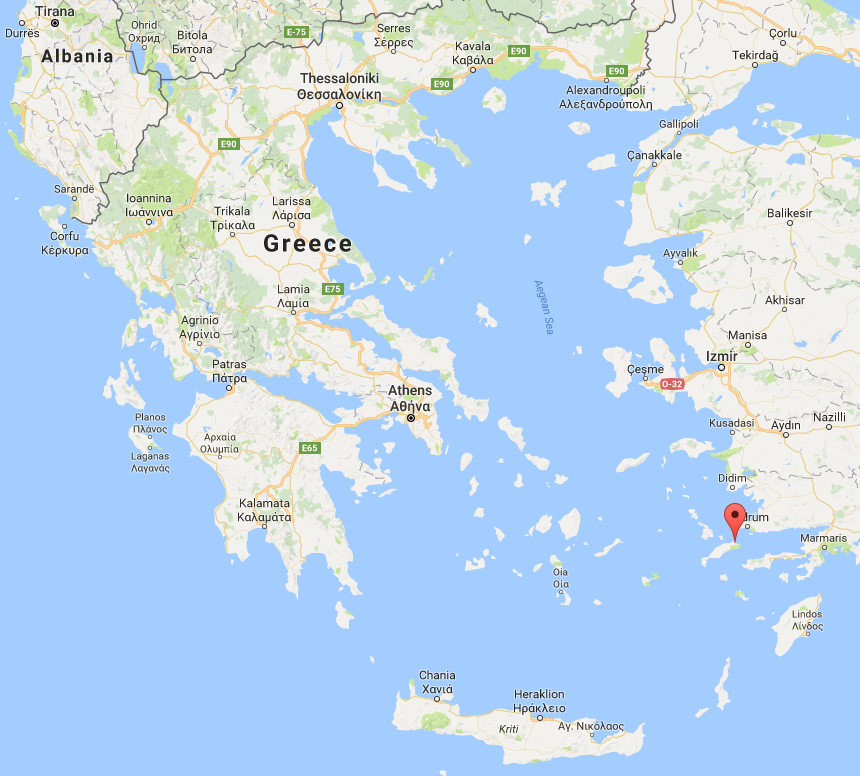
\includegraphics[width=\textwidth]{static/kos.png}
    \end{column}% 
    \begin{column}{.23\textwidth}
        
\includegraphics[width=\textwidth]{static/cardiff_uni_logo.jpg}

        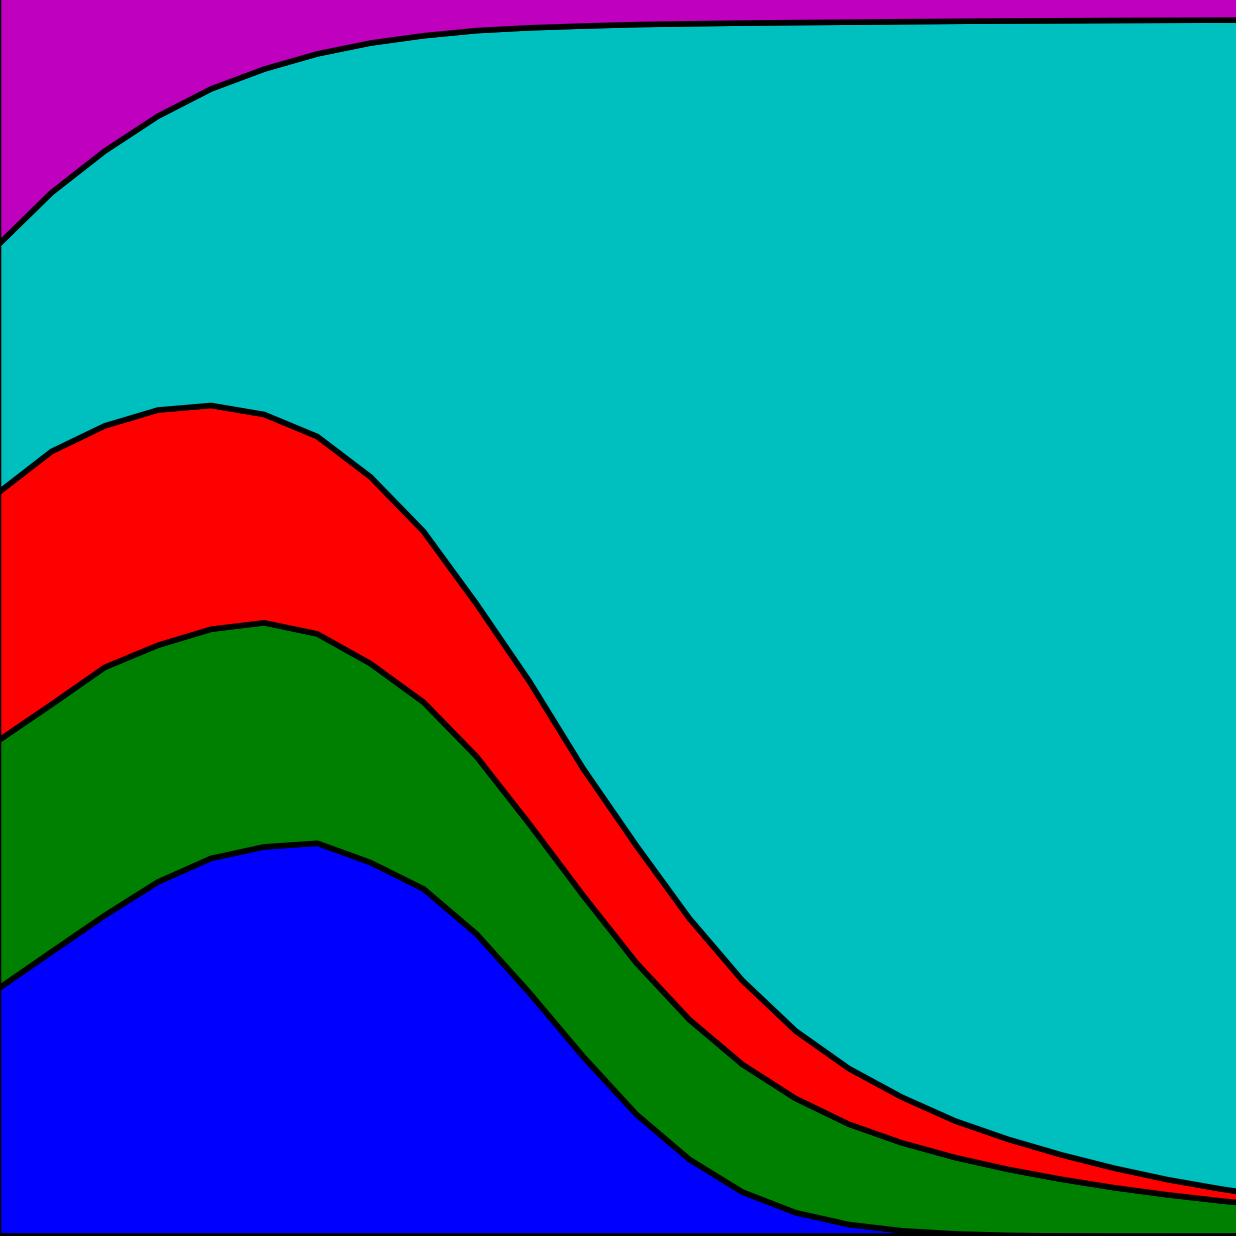
\includegraphics[width=\textwidth]{static/axelrod-logo.png}
    \end{column}%
    \begin{column}{.23\textwidth}
        
\includegraphics[width=\textwidth]{static/ssi-logo.png}

        
\includegraphics[width=\textwidth]{static/phoenix-logo.jpg}
\end{column}%
\end{columns}
\end{frame}

% A frame to explain the IPD
\begin{frame}
    \includestandalone[width=0.4\textwidth]{static/match/part_0}
\end{frame}
\begin{frame}
    \includestandalone[width=0.6\textwidth]{static/match/part_1}
\end{frame}
\begin{frame}
    \includestandalone[width=0.6\textwidth]{static/match/part_2}
\end{frame}
\begin{frame}
    \includestandalone[width=0.7\textwidth]{static/match/part_3}
\end{frame}
\begin{frame}
    \includestandalone[width=0.7\textwidth]{static/match/part_4}
\end{frame}
\begin{frame}
    \includestandalone[width=0.9\textwidth]{static/match/part_5}
\end{frame}

\begin{frame}
    \begin{center}
        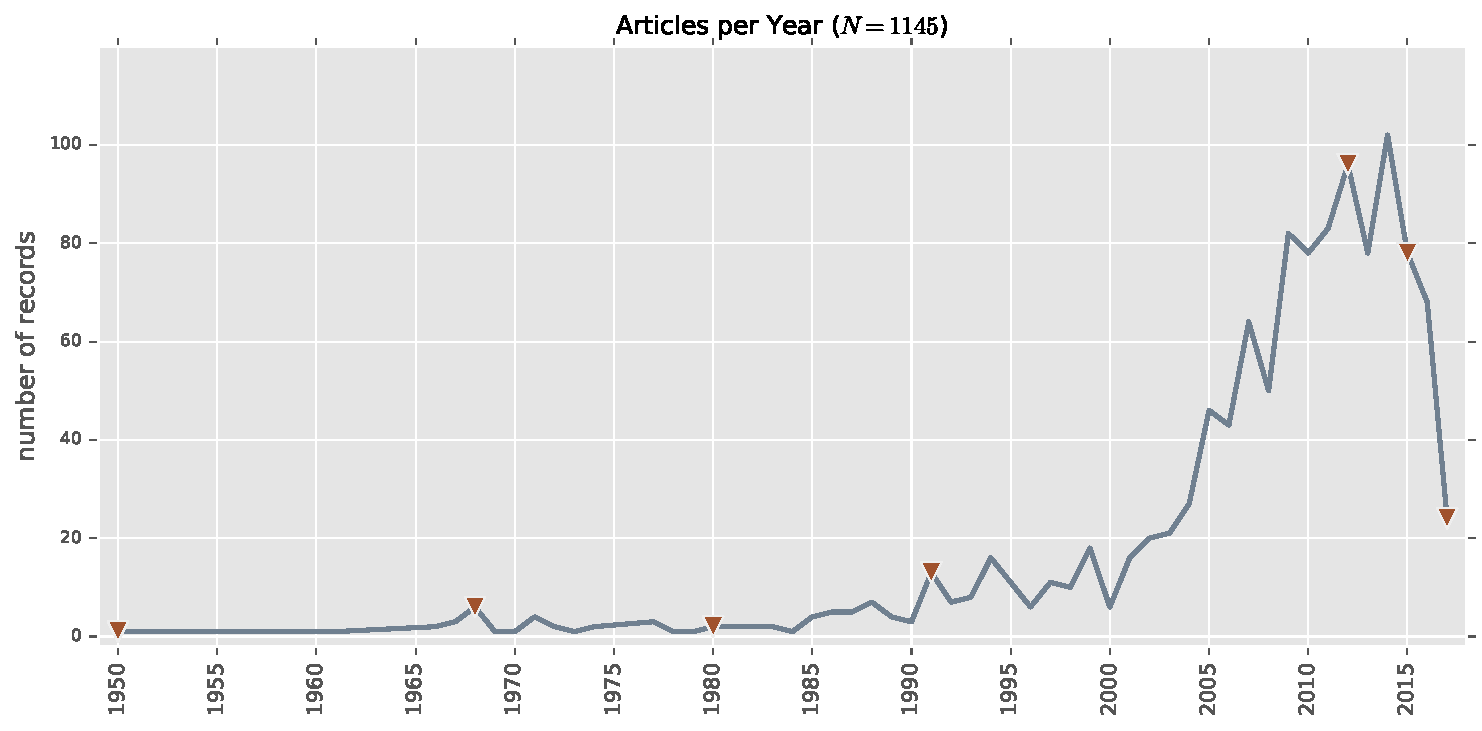
\includegraphics[width=\textwidth]{static/timeline.pdf}
    \end{center}
\end{frame}

\begin{frame}
    \begin{center}
        
\includegraphics[width=0.8\textwidth]{static/death_star.png}
    \end{center}
\end{frame}

\begin{frame}
\begin{columns}[T] % align columns
    \begin{column}{.5\textwidth}
        
\includegraphics[width=\textwidth]{static/shell.png}

        \end{column}% 
    \begin{column}{.6\textwidth}
        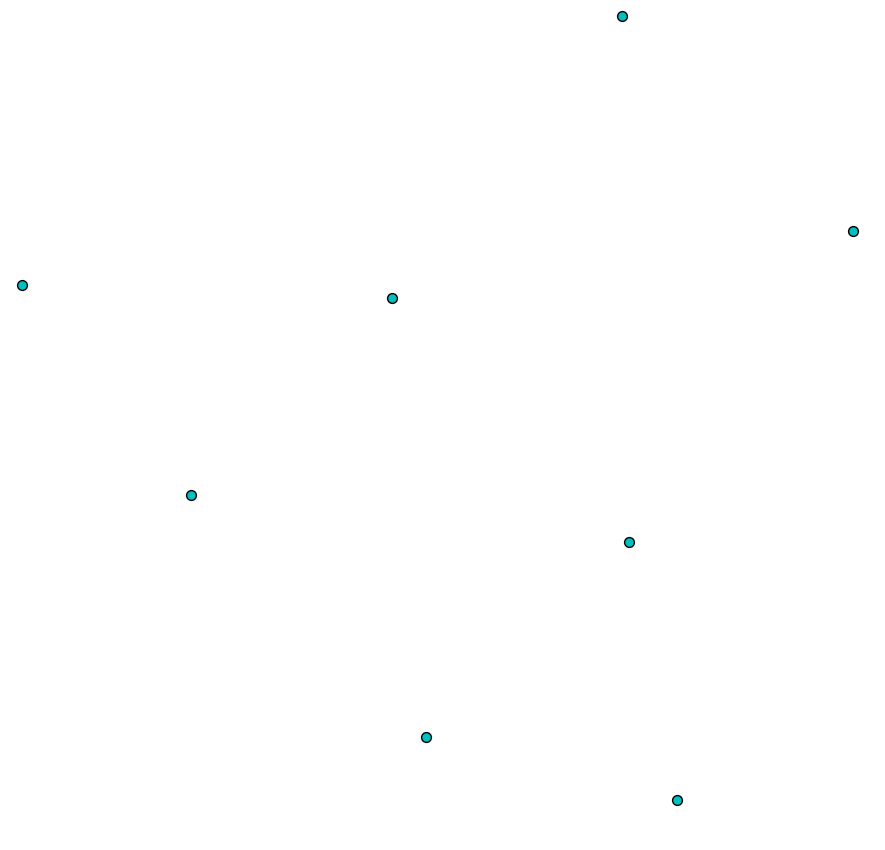
\includegraphics[width=\textwidth]{static/sedgewick.png}

       \vspace{-3cm} 
       \hspace{-2cm} 
\includegraphics[width=\textwidth]{static/diamond.png}
    \end{column}
\end{columns}
\end{frame}

\begin{frame}
\begin{center}
    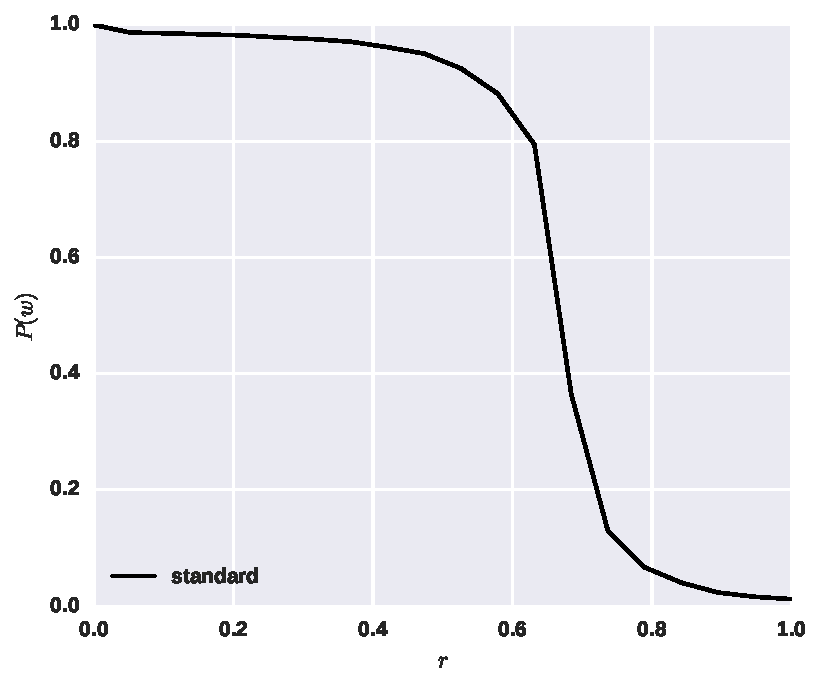
\includegraphics[width=0.48\textwidth]{static/standard.pdf}
    \hfill
    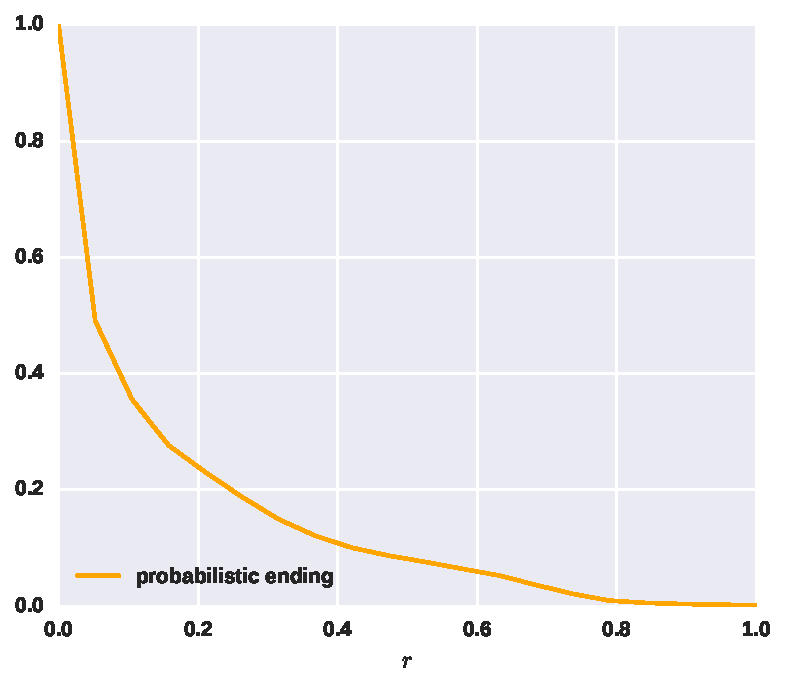
\includegraphics[width=0.48\textwidth]{static/probend.pdf}
\end{center}
\end{frame}

\begin{frame}
\begin{center}
    \includestandalone[width=0.6\textwidth]{static/memory_one_chain}
\end{center}
\end{frame}

\begin{frame}
    \begin{center}
       \begin{itemize}
        \item \textit{William Press and Freeman Dyson.} Iterated Prisoner’s
        Dilemma contains strategies that dominate any evolutionary opponent. 2012.
        \item  \textit{Christopher Lee, Marc Harper, and Dashiell Fryer.}
               The art of war: Beyond memory-one strategies in population games. 2015.
        \end{itemize}
    \end{center}
\end{frame}

\begin{frame}
    \begin{center}
        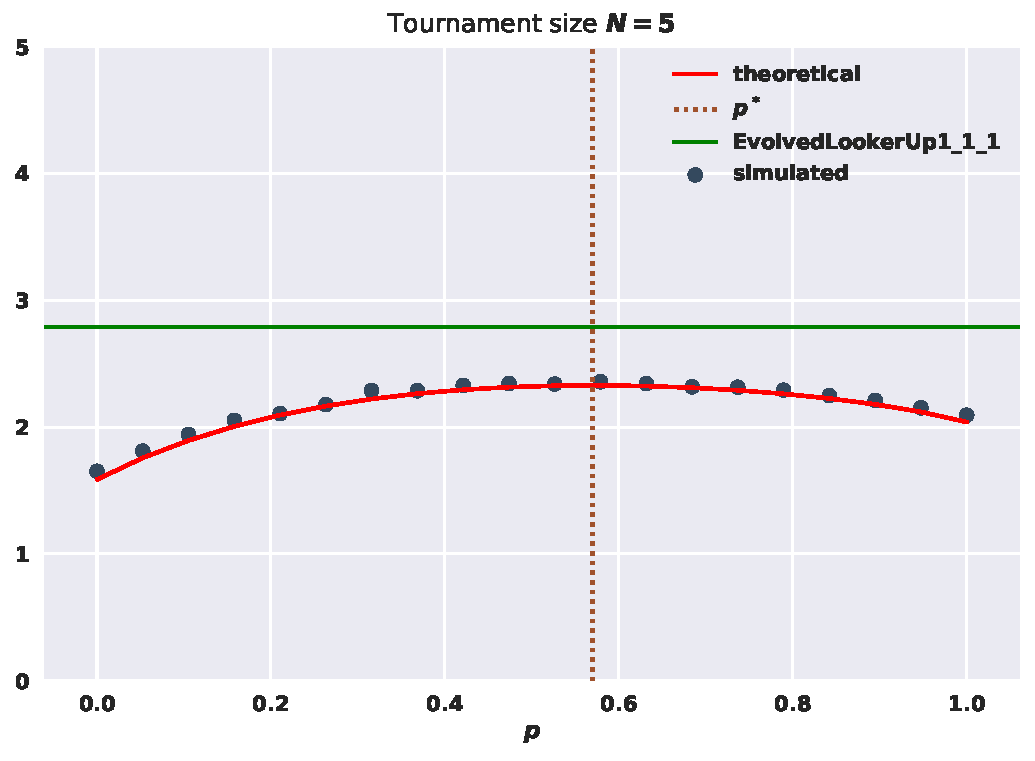
\includegraphics[width=0.8\textwidth]{static/optimisation.pdf}
    \end{center}
\end{frame}


\begin{frame}
    \begin{center}
        
\includegraphics[width=0.8\textwidth]{static/death_star.png}
    \end{center}
\end{frame}

\begin{frame}
    \begin{center}
        
\includegraphics[width=0.8\textwidth]{static/complex.png}
    \end{center}
\end{frame}

\end{document}

